\documentclass{article}[a4paper]
\usepackage[a4paper, total={6in, 9.5in}]{geometry}
\usepackage{charter}
\usepackage{xcolor}
\usepackage{graphicx}
\usepackage{float}
\usepackage{listings}
\usepackage{tabularray}
\usepackage{amsmath}
\usepackage{amssymb}
\usepackage{enumitem}
\usepackage{tikz}
\usepackage{pgfplots}
\usepackage{parskip}
\usepackage[hidelinks]{hyperref}

\setlength{\parskip}{0.75em}

\newcommand{\extlink}{
	
\begin{tikzpicture}[scale=0.1]
		\draw[rounded corners=0.5mm, line width=0.9pt] (-1, -1) rectangle (1, 1);
		\fill[white] (0, 0) rectangle (1.3, 1.3);
		\draw[line width=0.9pt, line cap=round] (0.15, 0.15) -- (1.3, 1.3);
		\draw[line width=0.9pt, line cap=round] (0.5, 1.3) -- (1.3, 1.3) -- (1.3, 0.5);
	\end{tikzpicture}
}

\lstset{
  language=Python,
  basicstyle=\ttfamily,
  keywordstyle=\color{blue},
  commentstyle=\color{gray},
  stringstyle=\color{red},
  showstringspaces=false,
  columns=fullflexible,
  breaklines=true,
  captionpos=b,
  backgroundcolor=\color[rgb]{0.96,0.96,0.96},
  xleftmargin=6pt,
  frame=tlbr,
  framesep=6pt,
  framerule=0pt,
  aboveskip=4pt,
  morekeywords={
    % NumPy
    numpy,np,array,arange,linspace,reshape,zeros,ones,empty,full,eye,random,randn,dot,linalg,mean,std,sum,min,max,argmin,argmax,
    % Matplotlib
    matplotlib,pyplot,plt,figure,subplots,plot,scatter,bar,hist,imshow,contour,title,xlabel,ylabel,legend,axis,grid,show
  }
}

\title{
	\huge{\textbf{
		Assignment 02
	}}\\
	\Large{
		Learning from Data, Related Challenges, Classification
	}\\
	\large{\phantom{}}\\
	\large{
		submitted for
	}\\
	\LARGE{
		\textbf{EN3150 - Pattern Recognition}
	}\\
	\large{
		Department of Electronic and Telecommunication Engineering
	}
	\\
	\large{University of Moratuwa}
}

\author{
	\textbf{Udugamasooriya P. H. J.}\\
	220658U\\
	\small{Progress on \href{https://github.com/pulasthi-u/en3150-assignment02}{GitHub \extlink}}
}

\date{20 August 2025}

\allowdisplaybreaks
\setlength{\parindent}{0pt}

\begin{document}
	\maketitle

	\section{Linear Regression}

	\textbf{Question 01} The main reason is the presence of outliers.
	
	Based on the inliers, we see that the desired line is an almost horizontal one. To see why a slanted line has been produced instead of a horizontal line, we look at the behavior of the squaring function;
	\begin{figure}[H]
		\centering
		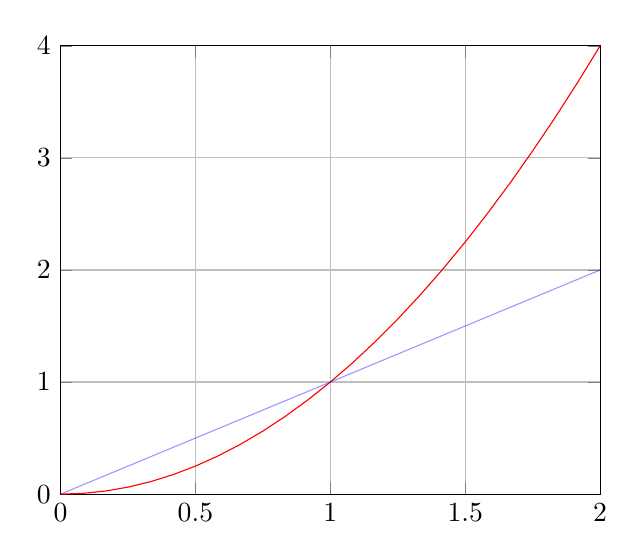
\begin{tikzpicture}
			\begin{axis}[
				xmin=0, xmax=2,
				ymin=0, ymax=4,
				grid,
			]
				\addplot[
					color=red,
					domain=0:2,
				]{x^2};
				\addplot[
					color=blue,
					opacity=0.4,
					domain=0:2,
				]{x};
			\end{axis}
		\end{tikzpicture}
		\caption{$y = x^2$}
	\end{figure}
	Note that for $|x| < 1$, $x^2 < |x| < 1$, i.e., the squares of numbers less than $1$ are less than the numbers themselves (in absolute value). This means that the squared loss function can remain small enough for prediction errors that are just slightly below $1$, but increases rapidly as it increases beyond $1$.

	In the given situation, even though a horizontal line would give near-zero error for the inliers, the error due to outliers would be very large. It is reasonable then, that a more optimal, i.e., with a lesser mean squared error, could be achieved with a slanted line,with lesser distance between outliers and the corresponding predictions.

	Such a line would increase the gap between the inliers and the corresponding predictions and therefore increase the loss, but \textit{not by too much}, due to the behavior of the square function. Instead, the reduction in the already-large gap between the outliers and the corresponding predictions, \textit{will} cause a \textit{rapid} decrease in the loss, \textit{exceeding} the increase in the loss due to the inliers.
	\medskip
	
	\textbf{Question 02} Scheme 1.
	
	The issue we wish to mitigate is the rapid increase in loss due to outliers, while keeping the loss due to inliers significant, with the intention that a model that better fits the inliers and is not strongly affected by the outliers as described above would be preferred.

	With Scheme 1, we do not completely neglect the effect of outliers, but significantly scale down their contribution to the loss function, so they do not dominate the loss when the loss due to the inliers is small.

	Scheme 2 is obviously not suitable, as it amplifies the loss from outliers over inliers; minimizing such a function would require the error due to outliers to be significantly reduced, causing more slanted line to be preferred, as described in the previous problem.
	\medskip
	
	\textbf{Question 03} In this case, the prediction to be made is of a categorical nature, i.e., a probability distribution over several possible classes, rather than a single continuous value.
	
	In linear regression, we try to fit a continuous linear model to a given set of data points. In doing so, we make the following assumptions:
	\begin{itemize}[noitemsep]
		\item the error between an actual data point and the corresponding prediction is normally distributed
		\item the data points vary continuously
	\end{itemize}
	However, in the case of categorical data, the variation of data points tends to be more discrete in nature, and the error between continuous-valued predictions and the data points is no longer normally distributed.

	More specifically, if each voxel is treated as a feature, we expect the data matrix $\mathbf{X}$ to have almost linearly dependent rows/columns, as we expect a high correlation between the voxels due to spatial smoothness in the images. This would lead to instability in the computation of $\left(\mathbf{X}^\top\mathbf{X}\right)^{-1}$ required for the ordinary least squares weights.

	On a final note, linear regression performs best when there are fewer features than data points for training. In our case, we expect the input images (data points) to consist of large numbers of voxels (features), but that there would be fewer such images than voxels. This might also lead to unstable coefficients, and sometimes overfitting, in the absence of regularization.

	\textbf{Question 05}
	\medskip

	\section{Logistic Regression}

	\textbf{Question 02} The following is a snippet of an error that was encountered:
	\begin{verbatim}
---------------------------------------------------------------------------
ValueError                                Traceback (most recent call last)

----> logreg.fit(X_train, y_train)

ValueError: could not convert string to float: `Adelie'\end{verbatim}

	The error indicates that not all data items given to \texttt{logreg.train} could be converted to the \texttt{float} data type. Clearly, all data \textit{must} be \textit{numeric} in order to enable the computation of weights and gradients required for logistic regression.

	The error arises from the line \lstinline|X = df_filtered.drop(['class_encoded'], axis=1)| in Listing 1 provided; \texttt{X} is prepared by dropping only the `\texttt{class\_encoded}' column, and therefore will retain the `\texttt{species}', `\texttt{island}', and `\texttt{sex}' columns from \texttt{df\_filtered}, whose entries are strings.

	In our case, `\texttt{species}' is not a feature---it is the label we intend to predict---and therefore mustn't even be contained in \texttt{X} at all.
	
	We have two options regarding `\texttt{island}' and `\texttt{sex}'; if we  believe the label we are trying to predict, i.e., the species of the penguin, depends on either of these features, then we could form \texttt{X} by replacing these columns with numerically encoded versions of them, or, if we believe they have little or no influence onf the label, we could drop them altogether.

	It is unlikely that the sex of a penguin has any influence on its species, so we will drop this feature entirely. A penguin's habitat (`\texttt{island}'), on the other hand, may be considered as influencing its species, as different species may have adaptations for different habitats. Whether or not to include it as a feature then depends on one's exact requirements. For the purposes of this problem, we will look at both options.
	
	Hence, we resolve the error as follows. We drop the `\texttt{species}' and `\texttt{sex}' columns entirely from `\texttt{df\_filtered}' to form \texttt{X\_}. Then, from \texttt{X\_} we form \texttt{X\_1} by one-hot encoding the contents of the `\texttt{island}' column and including them as new features, and \texttt{X\_2} by dropping the column entirely. The relevant lines of code are given in Listing \ref{errorfix}.

	\begin{lstlisting}[caption={Fix for the error}, label=errorfix]
X_ = df_filtered.drop(['species', 'sex', 'class_encoded'], axis=1)

# Form X_1 by one-hot encoding the island names and including them as new features
ohe = OneHotEncoder(sparse_output=False, drop='first', handle_unknown='ignore')
islands_encoded = ohe.fit_transform(X_[['island']])
X_1 = pd.concat(
    [
        X_.drop('island', axis=1).reset_index(drop=True),
        pd.DataFrame(islands_encoded, columns=ohe.get_feature_names_out(['island']))
    ], axis=1
)

# Form X_2 by simply dropping the 'island' column
X_2 = X_.drop(['island'], axis=1)
	\end{lstlisting}

	We then run the code given in Listing 2 to train the logistic regression model with both \texttt{X\_1} and \texttt{X\_2}. The outputs generated by each one respectively, are as follows:
	\begin{verbatim}
Accuracy : 0.5813953488372093
[[ 2.75836572e-03 -8.48924277e-05  4.43272550e-04 -2.85530563e-04
   1.84666104e-04 -1.04725548e-04]] [-8.62161382e-06]

Accuracy : 0.5813953488372093
[[ 2.76291513e-03 -8.24983988e-05  4.82711005e-04 -2.87644233e-04]]
 [-8.35428389e-06]
\end{verbatim}
	The same accuracy has been achieved in both cases, and the coefficients for common features in both cases are very similar. We further note that in both cases, the following warning was raised: \texttt{ConvergenceWarning: The max\_iter was reached which means the coef\_ did not converge}.
	\medskip

	\textbf{Question 03} It is clear that SAGA (Stochastic Average Gradient Ameliorated) has performed poorly on the current dataset, as indicated both by the relatively low accuracy of about $0.581$ on its performance on the data, and the fact that the coefficients did not converge.

	Being a stochastic method, SAGA performs best when the size of the dataset is large, ideally with more than tens of thousands of data points. This is because statistically, the gradient computed using a minibatch of the data points approaches the true gradient only when averaged over sufficiently many samples.

	Hence, the main reason for the poor performance of SAGA on our specific dataset is its size. Our dataset consists only of 214 data points---too few for SAGA to perform optimally.
	
	More specifically, we attribute the poor performance of SAGA to the following issues that may arise due to a dataset of this scale:
	\begin{itemize}[noitemsep]
		\item the gradient computation has a high tendency to be noisy
		\item a lot more iterations will be needed in order for any convergence to occur, as indicated by the \texttt{ConvergenceWarning}\item the overhead associated with each iteration is not ``offset" by a fewer number of iterations, as is usually the case with larger datasets
		\item sparsity?
	\end{itemize}
	\medskip
	
	\textbf{Question 04} The same code snippet in Listing 2 given was run using the `\texttt{liblinear}' solver in place of `\texttt{saga}' solver with training and test sets constructed using both \texttt{X\_1} and \texttt{X\_2} as described above, yielding respectively the following outputs;
	\begin{verbatim}
Accuracy : 1.0
[[ 1.51189823 -1.38940877 -0.14156163 -0.00378048  0.72408487 -0.5530247 ]]
 [-0.07450833]

Accuracy : 1.0
[[ 1.59665154 -1.42501103 -0.15238046 -0.003951  ]] [-0.0755452]
\end{verbatim}
	In each case, an accuracy of $1.0$ is reported.
	\medskip

	\textbf{Question 05} `\texttt{liblinear}' is a coordinate-descent method which uses all data points to compute the partial derivative with respect to a single coefficient at a time, and updates it over a number of iterations. Hence, it performs better on smaller datasets, with several hundreds of, or a few thousand data points, such as in our case.

	As such, `\texttt{liblinear}' does not incur as much overhead per iteration as a stochastic method such as SAGA. Thus, when the number of data points is small, it will converge faster than a stochastic method, with lesser memory and resource usage. Therefore, `\texttt{liblinear}' outperforms SAGA on our current dataset.
	\medskip

	\textbf{Question 06} The \texttt{random\_state} parameter passed to a \texttt{LogisticRegression} instance from \texttt{sklearn} controls how the coefficients will be initialized, and in the case of a stochastic method, how data points will be shuffled and selected randomly for iterations.

	Hence, performing different runs with different seed values for \texttt{random\_state} is expected to give different results and different accuracies, as each value would result in different coefficient initializations, and different minbatches of data points being used for updates.
	\medskip

	\textbf{Question 07} We implement standard scaling for the feature values and re-ran the logistic regression model with both `\texttt{liblinear}' and SAGA solvers. The results obtained are as follows:
	\begin{verbatim}
Accuracy with saga : 0.9767441860465116
[[ 3.90443923 -0.82356688  0.18543687 -0.73559796]] [-1.96731639]

Accuracy with liblinear : 0.9767441860465116
[[ 3.77819685 -0.75341497  0.17248526 -0.71597049]] [-1.72205563]
\end{verbatim}
	Equal accuracies of around $0.976$ are reported in both cases; a significant improvement over the previous value of $0.581$ with SAGA, but a marginal decrease compared to the previous value of $1.0$ with `\texttt{liblinear}'. We also note that both models have led to comparable coefficients.

	To see why this leads to a performance increase with SAGA, we note that standard scaling the features of the data points transforms them to be centered around zero, and restricts their variation along comparable scales. With stochastic methods such as SAGA, having all features on comparable scales helps stabilize gradient computation. Had this not been done, a randomly chosen minibatch may have features of a vastly different magnitude range than other batches, and therefore sudden variations/magnitude changes in the gradient, leading to uneven and haphazard steps being taken, slowing down convergence.

	Further, scaling ensures that the model learns to compare relative magnitudes \textit{across} features rather than be dominated by features that vary on very large scales, ignoring other features.

	In fact, the reason for the slight decrease in accuracy with `\texttt{liblinear}' with scaling may be due to the model starting to factor in other features more significantly; the previous accuracy of $1.0$ may have been due to some level of overfitting to the data, and it is possible that the model is now starting to exchange some of the lower bias it had previously achieved with a lower variance now, in an attempt to generalize better to unseen data.
	\medskip

	\textbf{Question 08} The stated approach is incorrect.
	
	Label-encoding a feature whose possible values are colors (with more than two colors) would imply some \textit{ordering} and relative \textit{weighting} among the colors, and is therefore unsuitable, unless such an ordering or weighting actually does exist (e.g., `green' - `least risk', `red' - `highest risk'/`twice as high a risk as green' etc.).
	
	Feature-scaling tends to preserve such an ordering and weighting. It would not address the problem of how exactly to assign labels to the colors.

	A more suitable approach would be to use one-hot encoding. Here, we treat each color as a binary-valued feature, and append them as extra features to the existing features. Doing so we avoid the implication of any form of ordering or weighting. Further, the values of these features will always be either $0$ or $1$, and therefore vary on comparable scales among each other.

	\section{First and Second Order Methods for Logistic Regression}

	\textbf{Question 02} We initialize weights by sampling randomly from a normal distribution.
	\medskip

	\textbf{Question 03} Loss function
	\medskip

	\textbf{Question 04} The implementation is given in Listing .
	\medskip

	\textbf{Question 05} The variation of the binary cross entropy loss over all the data points with the number of iterations with both batch gradient descent and Newton's Method is illustrated in Figure .

	Clearly, in both cases, the loss is decreasing with the number of iterations, indicating that the algorithm is indeed seeking an optimal set of weights. However, the loss decreases far more slowly with batch gradient descent, when compared with Newton's Method.
	\medskip

	\textbf{Question 06} Iterations
	\medskip

	\textbf{Question 07} Convergence
\end{document}